\documentclass[final]{beamer}

\mode<presentation>
  {
    \usetheme{Bright}
  }
  \usepackage{times}
  \usepackage{amsmath,amsthm, amssymb, latexsym}
  \usepackage{multirow}
  \usepackage[english]{babel}
  \usepackage[latin1]{inputenc}
  \usepackage[size=custom,width=120,height=85,scale=1.0,debug]{beamerposter} % dimension in centimeters

  %%%%%%%%%%%%%%%%%%%%%%%%%%%%%%%%%%%%%%%%%%%%%%%%%%%%%%%%%%%%%%%%%%%%%%%%%%%%%%%%%
  \graphicspath{}
  \title{Non-equilibrium umbrella sampling  on Blue Gene/P using one-sided communication}
  \author{Alex Dickson$^1$, Jeff R. Hammond$^2$ and Aaron R. Dinner $^1$}
  \institute{$^1$ The University of Chicago (\texttt{adickson@uchicago.edu,dinner@uchicago.edu}) \\ 
             $^2$ Argonne National Laboratory (\texttt{jhammond@alcf.anl.gov})}
  %%%%%%%%%%%%%%%%%%%%%%%%%%%%%%%%%%%%%%%%%%%%%%%%%%%%%%%%%%%%%%%%%%%%%%%%%%%%%%%%%

% ABSTRACT:
% In molecular simulations, important dynamics are often dominated by rare events. In such cases, reaction rates and transition states can be obtained by parallel sampling of phase space by regions. Nonequilibrium umbrella sampling (NEUS) is appropriate for systems driven far from equilibrium. In this poster we describe the first massively-parallel implementation of NEUS using Global Arrays. Efficient strong-scaling to 8192 processors of BlueGene/P is demonstrated for a coarse-grained, 262-residue RNA segment under explicit flow modeled with stochastic rotation dynamics. This approach can be used to scale explicit-atom molecular dynamics rare event simulations to many petaflops. Preliminary results show that the flow-extended RNA molecule can visit different meta-stable states, whose relative probabilities depend strongly on the pressure that drives the flow of the solvent. These developments suggest that the parallel version of NEUS will be a powerful tool to examine rare events in large nonequilibrium systems.

  \begin{document}

    \begin{columns}[t]

      \begin{column}{.33 \linewidth}

        \begin{block}{\Large Motivation} \Large
            Rare events pose a significant challenge for simulation since dynamics are simulated significantly slower than nature.  Much compute time is spent just waiting for the conditions to initiate an event.  Even under optimistic assumptions, some rare events will never be amenable to direct dynamics.
            \vskip-3ex
            \begin{columns}[t]
                \begin{column}{.5\linewidth}
                    \begin{eqnarray}
                        \tau_{MD}    & \approx & 10^{-15}~{\rm s} \\
                        \tau_{comp}  & \approx & 10^{-3}~{\rm s}
                    \end{eqnarray}
                \end{column}
                \begin{column}{.5\linewidth}
                    \begin{eqnarray}
                        T_{event}    & \approx & 10^{-6}~{\rm s} \\
                        T_{sim}      &    >    & 11~{\rm days}
                    \end{eqnarray}
                \end{column}
            \end{columns}
            \vskip1ex
            Non-equilibrium umbrella sampling (NEUS) replaces a sequential single dynamics trajectory with many trajectories which can be computed in parallel and is thus a massively-parallel algorithm for the time dimension of biomolecular simulation.
        \end{block}

	\begin{block}{\Large The Concept}
            \begin{columns}[t]
                \begin{column}{.44\linewidth}
                    Mountain climbing would be easy if it was broken up into pieces and each climber just had to cover one section, like a relay race.
                    \begin{figure}
                        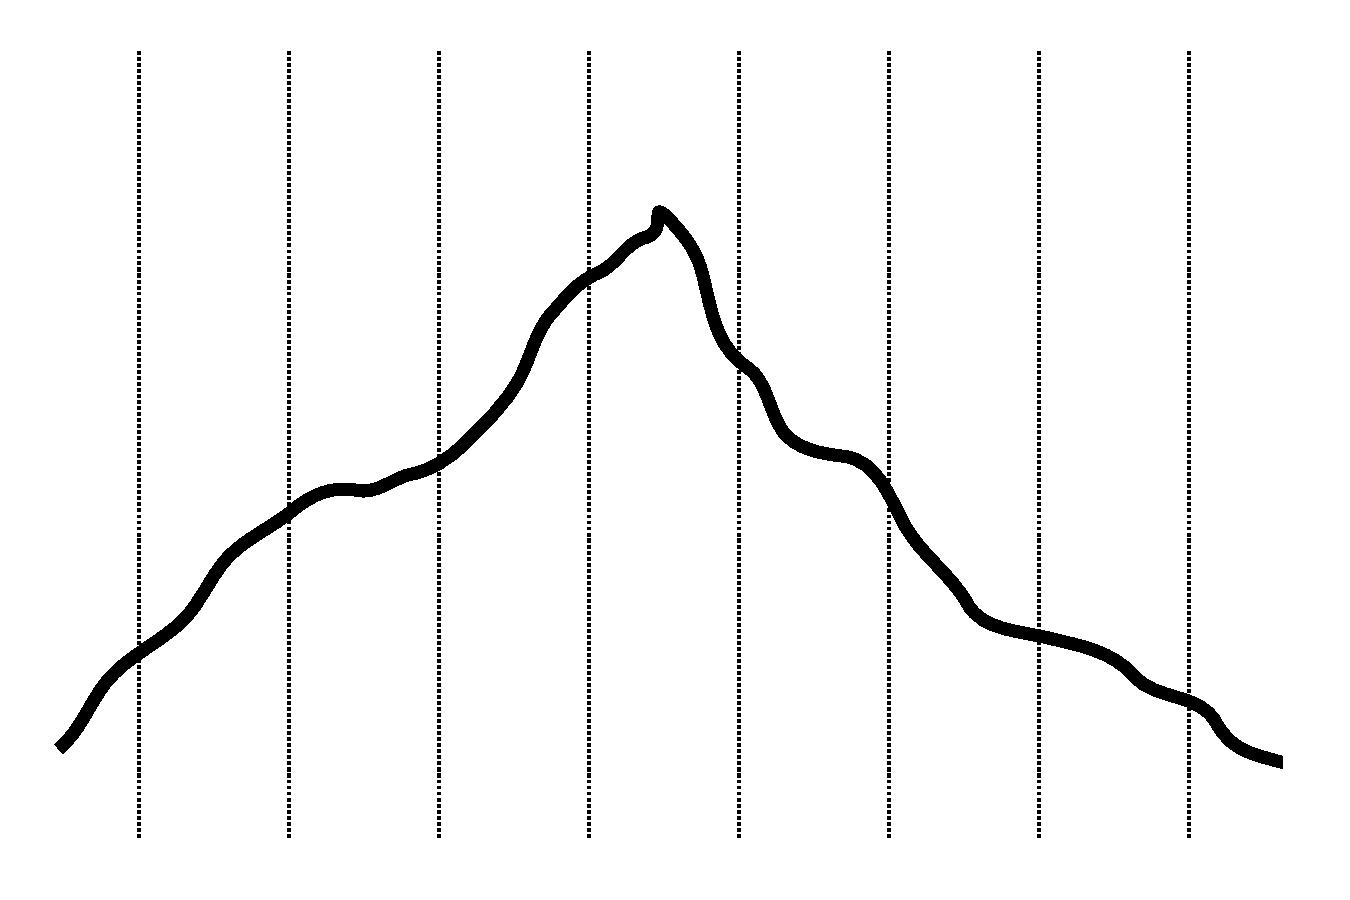
\includegraphics[scale=0.5]{images/mountain.pdf}
                    \end{figure}
                    Non-equilibrium umbrella sampling is a way to make molecular mountain climbing computationally tractable.
                \end{column}
                \begin{column}{.50\linewidth}
                    \begin{figure}
                        \includegraphics[scale=0.185]{images/DSCN4100.JPG}
                        %\includegraphics[scale=0.185]{/home/jeff/Documents/Posters/Supercomputing_2010/greg/DSCN4100.JPG}
                    \end{figure}
                \end{column}
            \end{columns}
	\end{block}

	\begin{block}{\Large How it works}\large
            NEUS samples an order parameter space using one or more degrees of freedom from the system that describe the relevant dynamics.  Many regions are sampled in parallel using independent simulations.   NEUS enforces sampling in every region of phase space, thereby simulating all stages of the event simultaneously and eliminating the wait time required to see a rare event.
            \begin{columns}[t]
                \begin{column}{.6\linewidth}
                    \centering
                    \begin{figure}
                        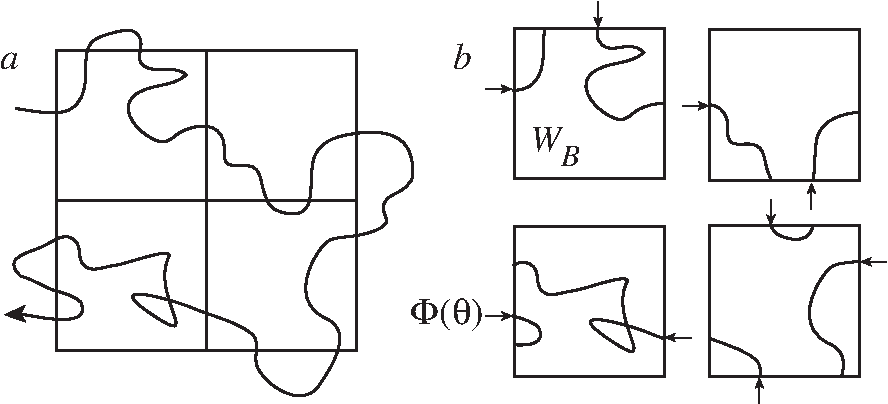
\includegraphics[scale=1.2]{images/motivation2.pdf}
                        \caption{Discretizing phase space.}
                    \end{figure}
                \end{column}
                \begin{column}{.4\linewidth}
                    \vskip-1ex
                    \begin{figure}
                        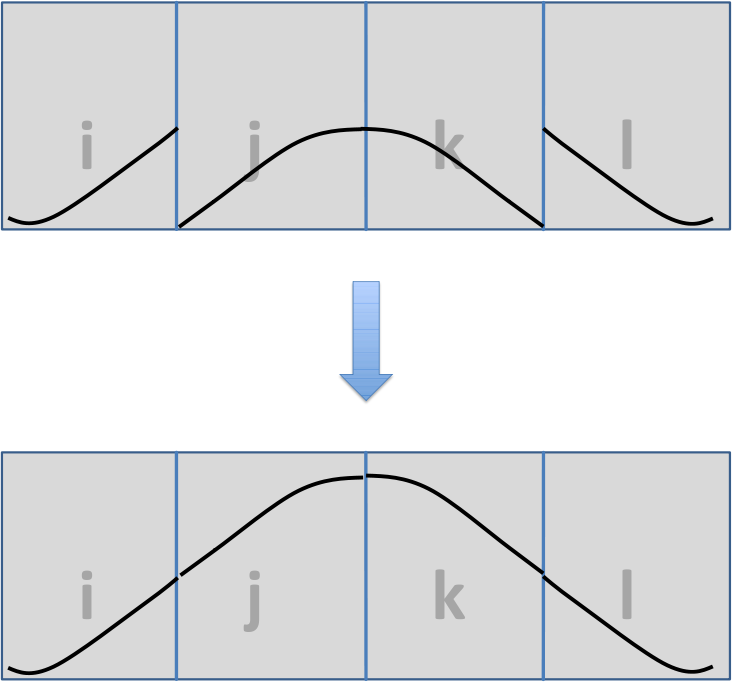
\includegraphics[scale=0.5]{images/patch.png}
                        \caption{Combining probabilities.}
                    \end{figure}
                \end{column}
            \end{columns}
            Each region is given a weight, that is determined using boundary crossing statistics.
            The weights are used to build the full steady-state distribution from the regional ones.
            \vskip1ex
            To conduct the ``regional'' simulations in nonequilibrium systems, one needs to be able to remove the bias in a physical way. The key insight is to run unbiased dynamics and restart walkers using a flux input distribution that is developed on-the-fly.
        \end{block}
      \end{column}

      \begin{column}{.32 \linewidth}

%           The NEUS algorithm provides a massively-parallel method to obtain important information about rare event dynamics in complex systems.  The scalability of NEUS \textit{improves} for larger systems since the time spent on an individual sample.  Application of NEUS to proteins modeled with explicit-atom force-fields (instead of the simple bead model considered here) would scale to many thousands of times the number of processors required for the molecular dynamics (MD) evaluation.  Given the scalability of MD codes like LAMMPS and NAMD, it is reasonable to project near-exascale simulation of rare events in proteins using explicit-atom models.
%         \end{block}

	\begin{block}{\Large Nonequilibrium Umbrella Sampling in Detail}\large
            NEUS is an umbrella sampling algorithm that is applicable to nonequilibrium systems.  It divides the phase space of a system into different regions and conducts restricted simulations within each region.
            \vskip1ex
            \textbf{Strings:}
            \begin{columns}[t]
                \begin{column}{.42\linewidth}
                    Irregular regions can be formed by Voronoi polyhedra defined using a set of phase space points (``images'') that together form a string that winds its way from reactants to products.  The string is updated during sampling by periodically moving the images towards the average of the walker position in the last time interval.
                \end{column}
                \begin{column}{.48\linewidth}
                    \vskip-3ex
                    \begin{figure}[hcts]
                        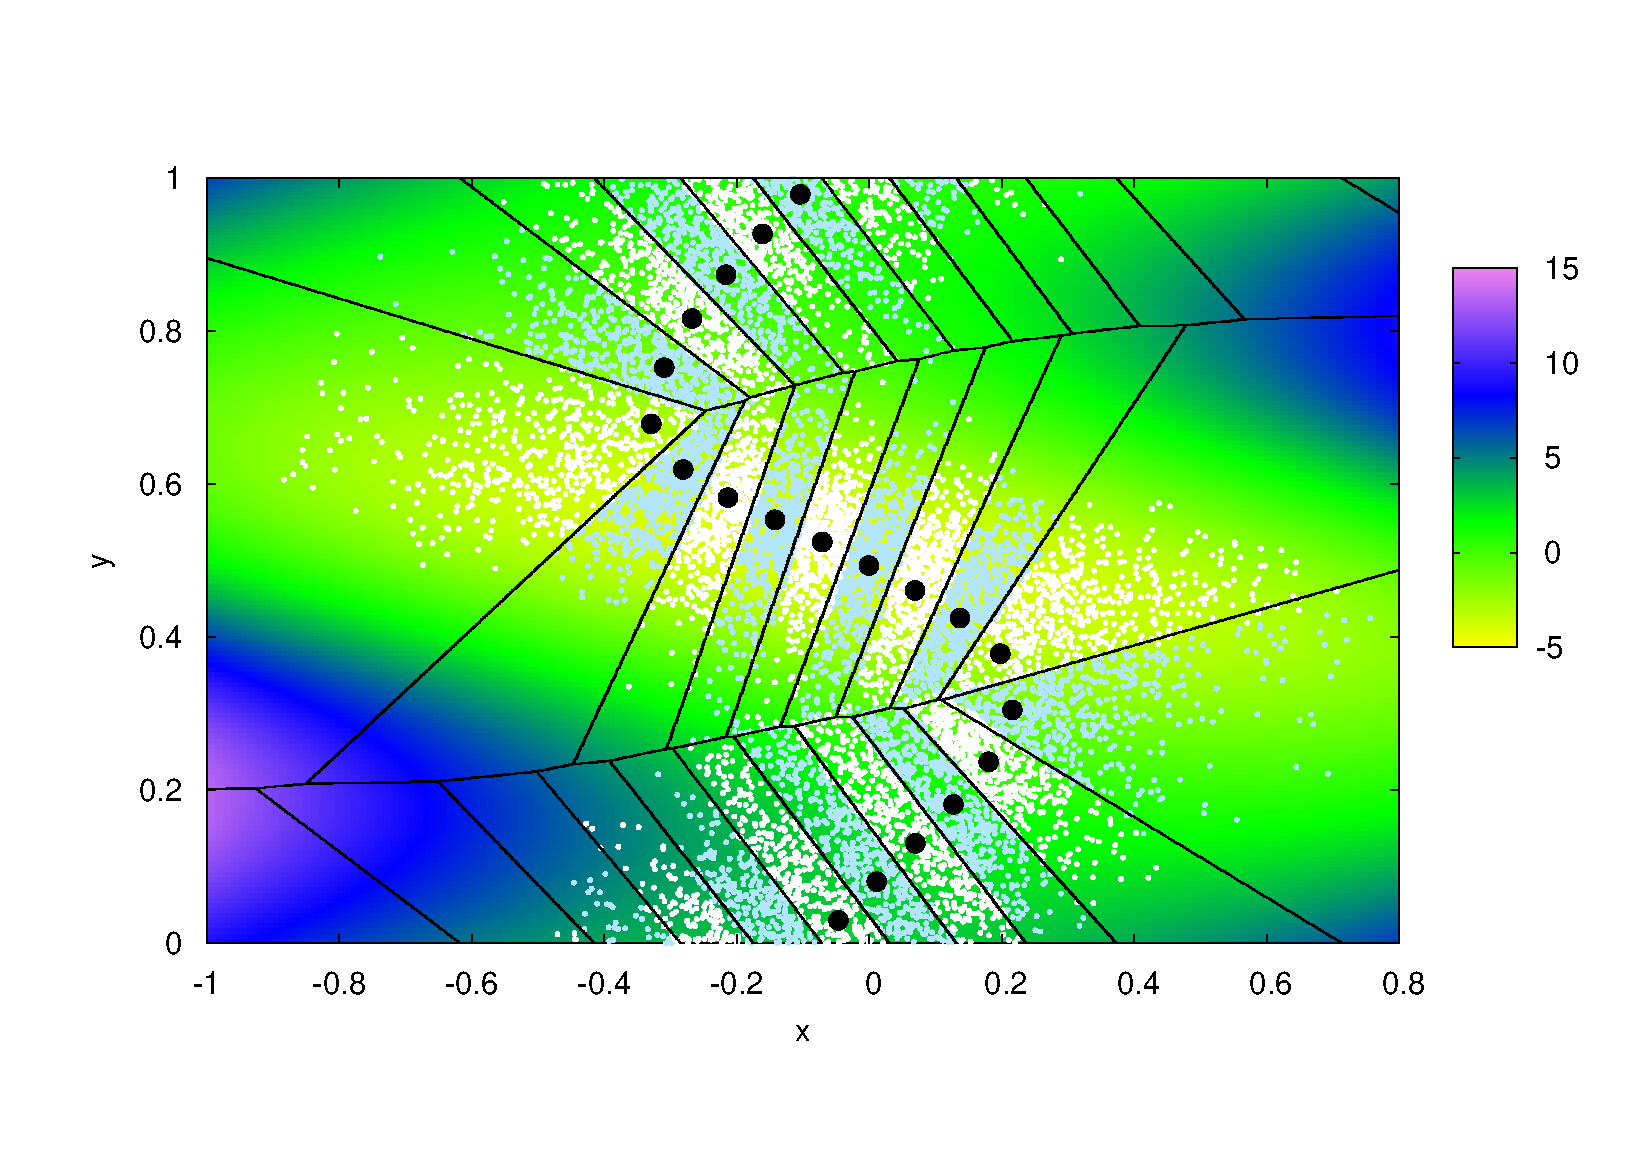
\includegraphics[width=1.0\linewidth]{images/whiteandblue.pdf}
                    \end{figure}
                \end{column}
            \end{columns}
            \vskip2ex
            \textbf{Separating the transition path ensemble:}
            \begin{columns}[t]
                \begin{column}{.50\linewidth}
                    We can also separate trajectories based on their basin of origin by defining two ensembles:  ${\cal S}_A$ for trajectories originating in basin $A$, and ${\cal S}_B$ for trajectories originating in basin $B$.  This allows for a better description of transition paths that are separate due to nonequilibrium path splitting, and as a bonus, it allows for the \textbf{easy calculation of transition rates!}
                    \begin{equation*} \label{eq:rate}
                        k_{AB} = \frac{\overline{\Phi}_{B \mid {\cal S}_A}}{\overline{h}_A}
                    \end{equation*}
                    where $\overline{\Phi}_{B \mid {\cal S}_A}$ is the flux into basin $B$ from the ${\cal S}_A$ ensemble, and $\overline{h}_A$ is the total weight of all regions in ${\cal S}_A$.
                \end{column}
                \begin{column}{.40\linewidth}
                    \vskip-5ex
                    \begin{figure}
                        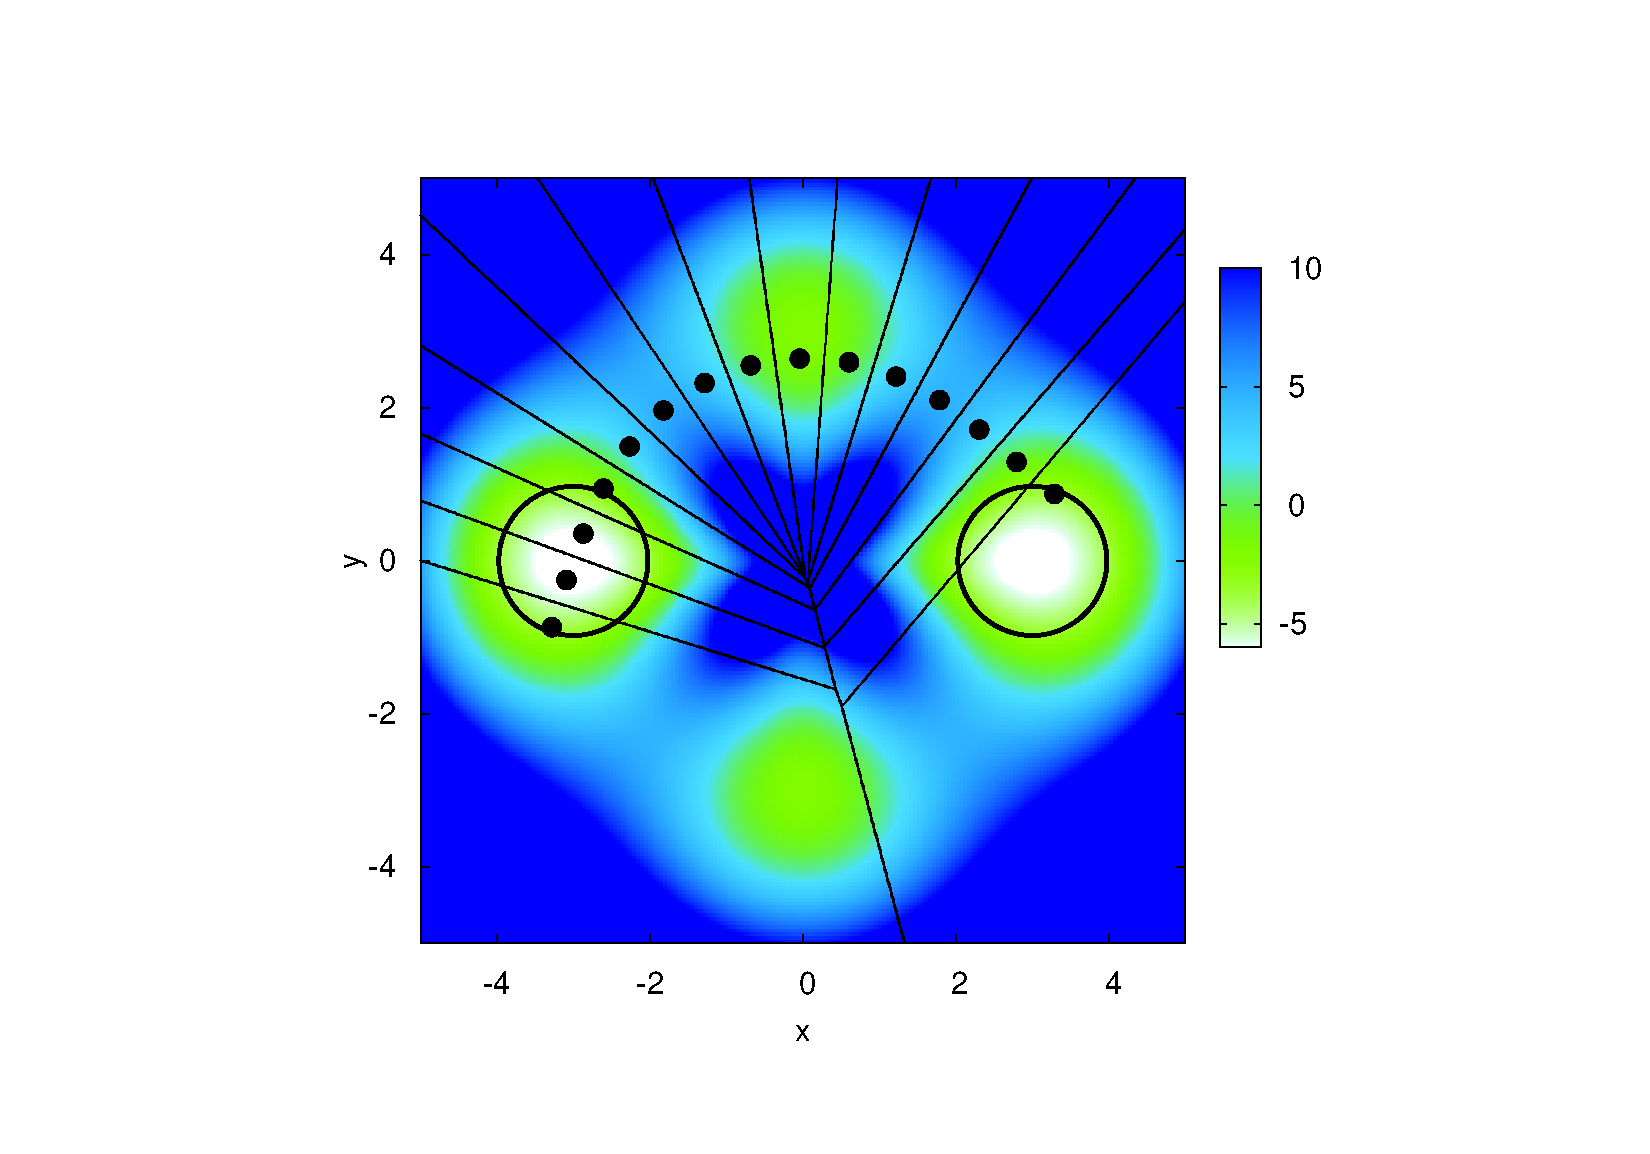
\includegraphics[width=1.0\linewidth]{images/contvorf.pdf}
                    \end{figure}
                    \begin{figure}
                        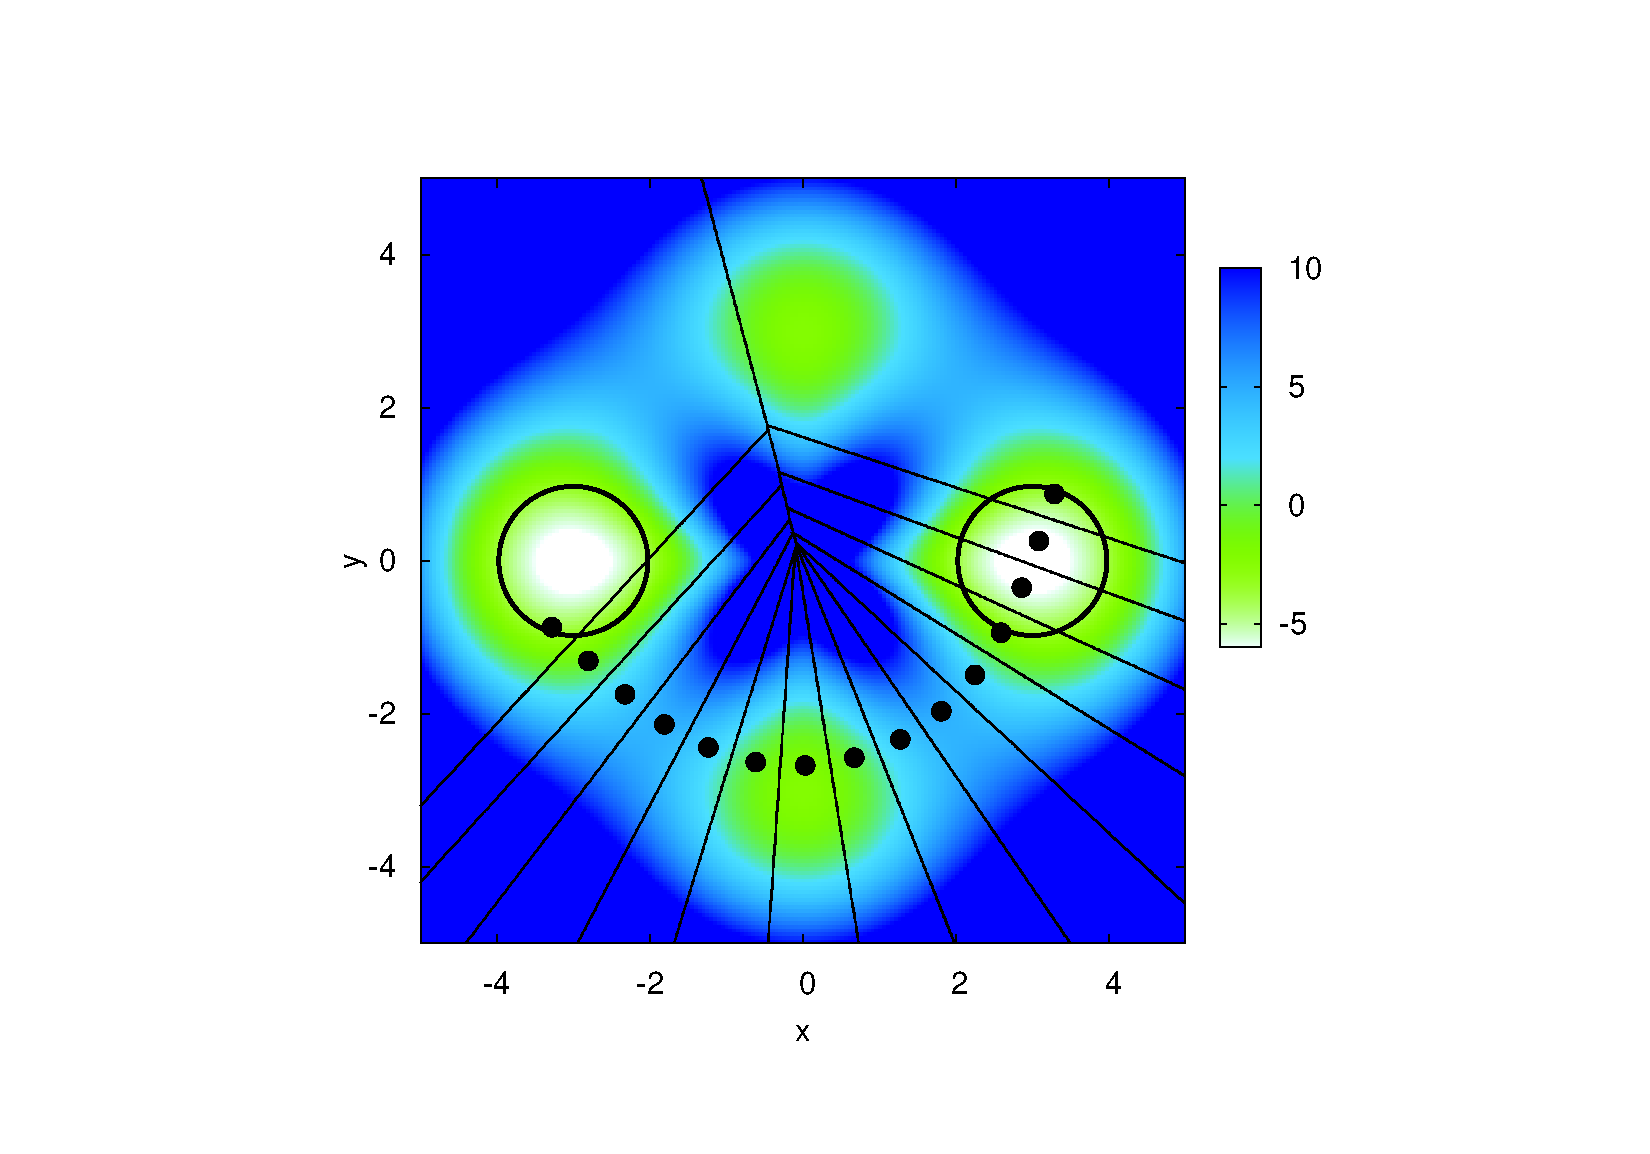
\includegraphics[width=1.0\linewidth]{images/contvorr.pdf}
                    \end{figure}
                \end{column}
            \end{columns}

        \end{block}

            \begin{block}{\Large Algorithmic and Implementation Efficiency}\large
                \begin{columns}[t]
                    \begin{column}{.48 \linewidth}
                        NEUS outperforms FFS when long-lived intermediate states are present.  Both methods outperform conventional sampling when the transitions are sufficiently rare.
                    \end{column}
                    \begin{column}{.48 \linewidth}
                        The distributed nature of the NEUS global state allows for efficient strong-scaling due to the majority of asynchronous updates being nonconflicting. 
                    \end{column}
                \end{columns}
                \vskip1.5ex
                \begin{columns}[t]
                    \begin{column}{.48 \linewidth}
                        \begin{figure}[hcts]
                            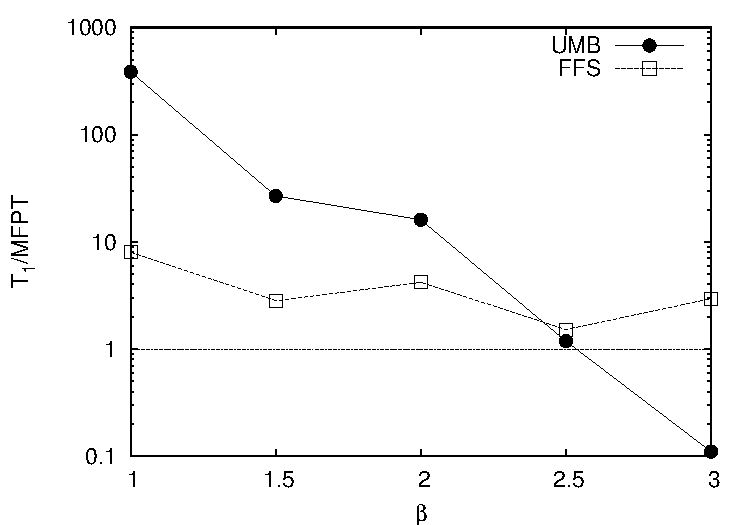
\includegraphics[width=0.9 \linewidth]{images/master.pdf}
                            \caption{Efficiency results from the circular model potential, where $\beta$ is the inverse temperature. Transitions become more rare as $\beta$ increases.}
                        \end{figure}
                    \end{column}
                    \begin{column}{.48 \linewidth}
                        \begin{figure}[hctp]
                            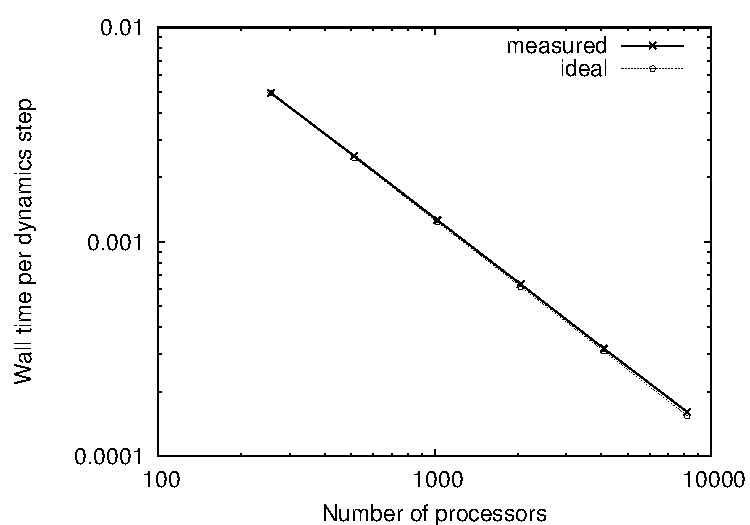
\includegraphics[width=0.9 \linewidth]{images/scale.pdf}
                            \caption{Strong scaling to 8192 cores with 96\% efficiency.}
                        \end{figure}
                    \end{column}
                \end{columns}
            \end{block}

      \end{column}

      \begin{column}{.33 \linewidth}

% coordserver contains a family of functions that create coordinate servers, and perform GA puts and gets.  the creation functions were not modified from the ones you gave me except I made two separate ones, one for double and one for ints.  The puts and gets are slightly more easy-to-use versions of NGA_Get and NGA_Put that return either a single value of a 2D array (I made all of my arrays 2-dimensional, with the first limit being 2, just because all of them were of that form anyway...), or, if the second array index is -1, return a whole half of the array.  Later on as I became more comfortable I started calling the NGA_Gets and puts directly, when I needed the whole array, that way I wouldn’t have to call it twice

        \begin{block}{\Large Parallelization using Global Arrays}\large
            NEUS is implemented using a global state updated by atomic (complex) operations asynchronously.  Global Arrays (GA) Put/Get operations in conjunction with Lock/Unlock provide a means to implement the necessary tools in a straightforward way.  The implementation of NEUS on top of GA is called CoordServer.
            \begin{columns}[t]
                \begin{column}{.48 \linewidth}
                    \begin{figure}[hctp]
                        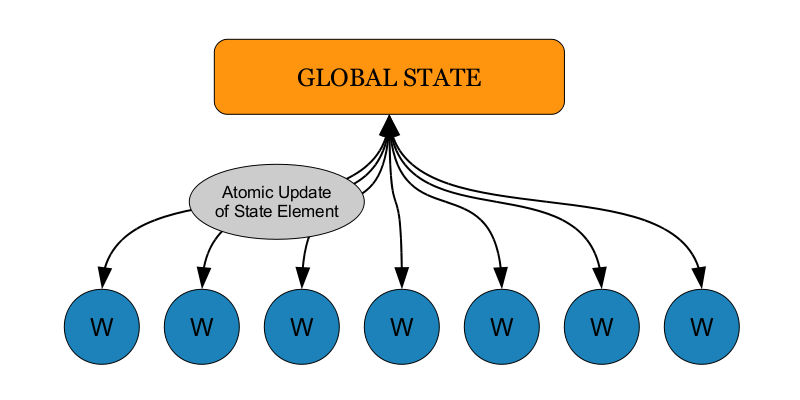
\includegraphics[width=1.0\linewidth]{images/soft_arch.png}
                    \end{figure}
                \end{column}
                \begin{column}{.48\linewidth}
                    \begin{figure}[hctp]
                        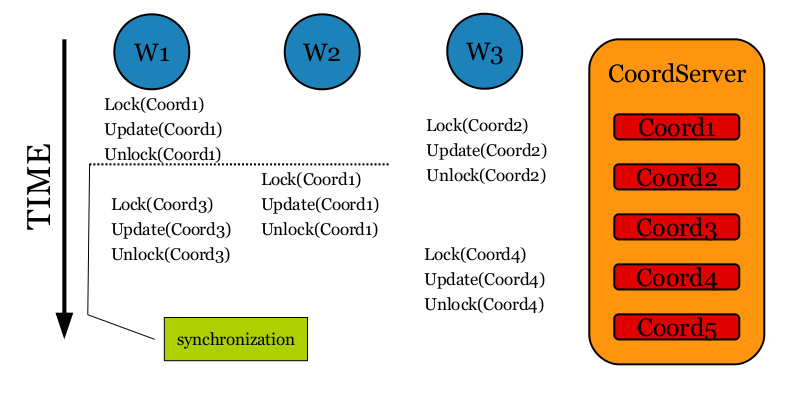
\includegraphics[width=1.0\linewidth]{images/coord_server.png}
                    \end{figure}
                \end{column}
            \end{columns}
            Because Global Arrays provides a \textit{distributed} global state, atomic updates can occur simultaneously except when locked.  A master-worker approach would force unnecessary serialization of updates.
        \end{block}

        \begin{block}{\Large Results for RNA}\large
            \textbf{Evidence for long-lived stable-states}: The competition between the flow and the native contacts results in a rich dynamics that includes competing metastable states.  We are interested in the intermediate case, where contracted and extended states coexist, and transitions between them occur on long, macroscopic timescales.
            \vskip1ex
            \begin{figure}[hctp]
                \vskip-5ex
                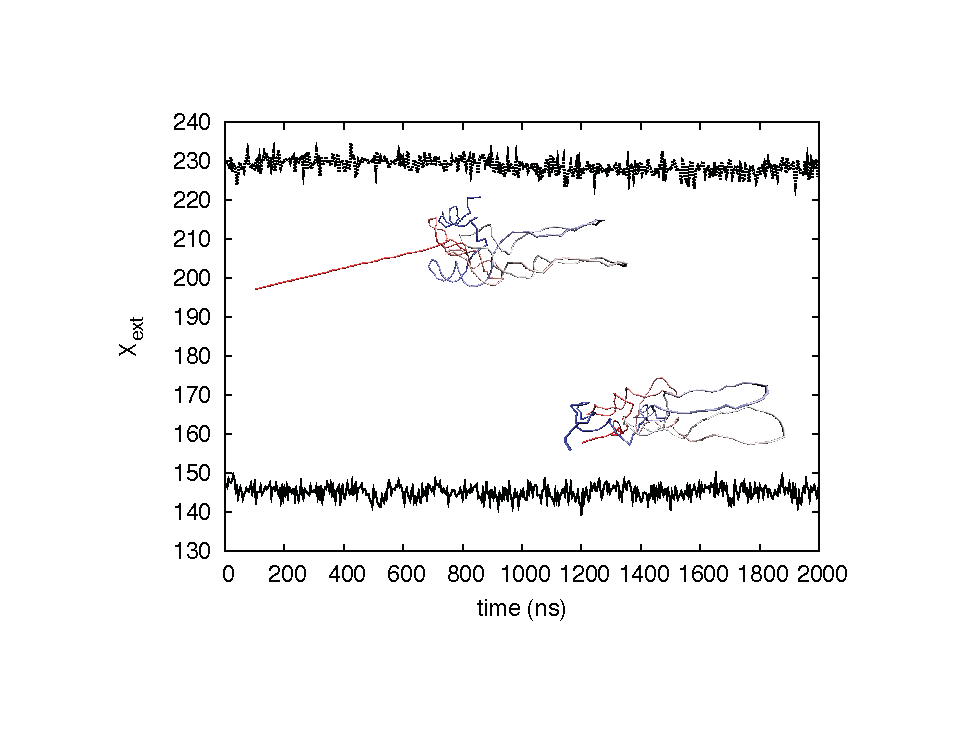
\includegraphics[width=0.79 \linewidth]{images/ext_fig.pdf}
                \vskip-5ex
                \caption{Extension vs. time for two trajectories with different initial conditions.}
            \end{figure}
            \vskip1ex
            \textbf{Problem Description:}  Each of the 262 nucleotides is represented by a single bead.  Adjacent beads in the chain are connected with a FENE potential, and secondary and tertiary interactions are modelled with a Lennard-Jones potential.  Repulsive terms keep the chain local straight to mimic steric repulsion.  The flow is simulated with the stochastic rotation dynamics method.
            \vskip1ex
            Flow is simulated with the stochastic rotation dynamics wherein solvent is represented by a large number of infinitesimal particles that are grouped into cells of a lattice.  Each step of the algorithm is comprised of a free streaming step and a ``collision'' step in which the velocity of each particle in the cell is rotated around the cell's average velocity vector by a random rotation matrix.  The RNA beads are included in the collisions, through which the solvent will influence the polymer.
        \end{block}

      \end{column}

    \end{columns}

  \end{document}